% sci.tex - SCI STYLE FILE 使用例

\documentclass{jarticle}
\usepackage{sci}

\usepackage[dvipdfmx]{graphicx}
\usepackage{txfonts}
% 日本語原稿の場合
% 
% LaTeX2e
% \documentclass{jarticle}
% \usepackage{sci}
% 
% LaTeX209
% \documentstyle[sci]{jarticle}

% 英語原稿の場合
% 
% LaTeX2e
% \documentclass{article}
% \usepackage{latexsym}
% \english
% 
% LaTeX209
% \documentstyle[sci]{article}
% \english

% 2006-11-16 modification by TF %SCI07

\jtitle{深層学習を用いた人狼エージェントの行動予測}
\etitle{The Behavior Prediction of Werewolf Game Agents by Use of Deep Learning}
\jauthor{大阪府立大学 \ ○ \ 近藤 \ まなみ,松本 \ 啓之亮,森 \ 直樹}
\eauthor{Manami Kondoh,Keinosuke Matsumoto,Naoki Mori\\ 
  Osaka Prefecture University}
\englishabstract{Recently,incomplete information game is attracting attention in the field of game research.In incomplete information game,we have  only missing information.Therefore we must act based on the prediction in order to calculate optimum solution.Werewolf Game is a kind of incomplete information game,and  classified as a communication game.There are theory or trend of each player in that game.In this research,we aim to predict 'vote' of Werewolf Game by learning those features from game logs.}
%近年,ゲーム研究の分野で不完全情報ゲームが注目を集めている.不完全情報ゲームはその性質により,最適解を得るためには予測に基づいて判断する必要がある.人狼ゲームは不完全情報ゲームの一種であり,コミュニケーションゲームに分類され,プレイヤごとの定石や傾向が存在する.本研究では,人狼ゲームのゲームログを用いてその傾向などを学習することで,プレイやの投票先を予測することを目的としている.

\begin{document}

\maketitle

\section{はじめに}
ゲームAIの分野において,これまで将棋や囲碁などの(二人零和有限確定)完全情報ゲームに関する研究が数多くなされてきた結果,必勝法の発見や熟練したプレイヤに勝利するAIエージェントの実現という成果が得られた.そして近年,ゲームAI研究の対象として,麻雀やポーカーなどの不完全情報ゲームが注目を集めている.不完全情報ゲームは情報に不足や不確実性がある,運や確率に依存するなどの課題から,前者のような成果はまだ得られていない.このような課題を踏まえたうえで最適解を得るためには,予測に基づいて判断する必要がある.\par
人狼ゲームは複数人で行うコミュニケーションゲームの一種であり,不完全情報ゲームに分類される.このゲームにおいてプレイヤが得られる情報は制限されており,与えられた情報には虚偽が混在していることがある.\par
本研究では,人狼ゲームにおいて制限された情報から定石やプレイヤごとの傾向を学習することで,不確定な情報下での予測精度を向上させることを目的としている.人狼ゲームにおいて取れる行動は,'発言','投票','能力行使'が挙げられるが,本稿ではその中のひとつ'投票'に焦点を当て検討する.\par
利用可能な情報のみを用いて投票先を予測するためには,その情報と投票先との関連性に着目しなければならない.そこで,その関連性を学習するために深層学習(Deep Learning)を用いる.また,人狼ゲームは時間経過とともに情報が増える,過去の発言が現在に影響するなど,時系列性を有するゲームである.そこで,その時系列性を考慮するために再帰型ニューラルネットワークの一種であるLSTM(Long Short-Term Memory)\cite{LSTM}という手法を導入する.\par

\section{人狼ゲーム}
人狼ゲームとは,村人陣営と人狼陣営に分かれて自陣の勝利を目指すゲームである.村人陣営は人狼を全滅させること,人狼陣営は人間を人狼と同数以下にすることが勝利条件となっている.村人陣営はプレイヤ同士の会話などから人狼を見破る必要があり,人狼は村人に見破られないように振舞わなければならない.\par
以下に,本研究で取り扱う人狼ゲームの概要および設定を示す.

\subsection{進行}
ゲームはTalk,Vote,Actionの順で進行する.これが1日の流れであり,1日が終了すると勝利判定がされ,どちらかの陣営が勝利条件を満たしていれば終了,満たしていなければ死亡者をゲームから排除して再びこの3フェーズを繰り返すこととなる.\\
\vspace{-1.5\baselineskip}
\begin{itemize}
\setlength{\leftskip}{-1zw}
  \setlength{\parskip}{0cm}
  \setlength{\itemsep}{0cm}
 \item Talk(会話)\\ 
プレイヤ同士が会話をする.情報の交換や推理,または誰を処刑するかの話し合いをするフェーズとなる.
 \item Vote(投票)\\
各プレイヤが処刑したいプレイヤに投票する.投票の結果,得票数が最多の者が処刑される.同票の場合は得票数最多者の中からランダムに選ばれる.
 \item Action(能力行使)\\
特殊能力を持つプレイヤが能力を行使する.行使対象や結果は当事者にしか開示されない.
\end{itemize}

\subsection{役職}
人狼ゲームでは各プレイヤに役職が振り分けられる.役職にはそれぞれ異なる役割や能力があり,プレイヤがどの役職に振り分けられたかは当事者にしかわからない.以下に,本稿で扱う役職の種類と能力を示す.\\
%\vspace{0.3\baselineskip}
%\\
【村人陣営】\\
\vspace{-1.5\baselineskip}
\begin{itemize}
\setlength{\leftskip}{-1zw}
  \setlength{\parskip}{0cm}
  \setlength{\itemsep}{0cm}
\item 村人(VILLAGER)\\
特殊能力を持たない役職.Actionフェーズでは行動しない.
\item 占い師(SEER)\\
プレイヤを1人選択することで,そのプレイヤが人狼であるか否かを知ることができる.
\item 霊媒師(MEDIUM)\\
処刑者が人狼であったか否かを知ることができる.
\item 狩人(BODYGUARD)\\
プレイヤを1人選択することで,そのプレイヤを人狼の襲撃から護ることができる.
\end{itemize}
【人狼陣営】\\
\vspace{-1.5\baselineskip}
\begin{itemize}
\setlength{\leftskip}{-1zw}
  \setlength{\parskip}{0cm}
  \setlength{\itemsep}{0cm}
\item 人狼(WEREWOLF)\par
プレイヤを1人選択することで,そのプレイヤを襲撃し,ゲームから排除させることができる.人狼同士はゲーム開始時に互いが人狼だと認識することが可能なため,意図せず仲間を投票や襲撃対象に選択してしまうことは回避できる.
\item 狂人(POSSESSED)\par
特殊能力をもたない役職.Actionフェーズでは行動しない.人狼側のプレイヤであるが占いや霊媒対象となったときは人間であるという結果になり, 勝敗条件では村人側としてカウントされる.
\end{itemize}

\subsection{設定}
本研究では人狼をプレイするAI,いわゆる人狼知能\cite{aiwolf}によるゲームを対象としている.人狼知能プロジェクト\cite{project}で公開されているプラットフォームver 0.3.5を用いると,エージェント同士による人狼ゲームが実行できる.本稿ではこのプラットフォームver 0.3.5の設定を用いる.このゲームにおいて,Talkフェーズで発話可能な内容や回数は制限されている.表\ref{tb:talk}にゲーム中で可能な発言種類を示す.\par
実際にゲームをプレイするエージェントセットには,第二回人狼知能大会で決勝14位に入賞した「JuN1ro」を用いる.JuN1roは各役職ごとに異なるアルゴリズムを持つ.また,行動は基本的に内部の人狼予測関数に基づき決定するため,投票先をランダムに決定することはない.\par
ゲームは村人8人,人狼3人,占い師,霊媒師,狩人,および狂人1人のJuN1roで構成する15人村を想定する.

%\setlength\textfloatsep{5pt}
 \begin{table}[t]
 \caption{ゲーム内で可能な発言種類 \label{tb:talk}}
 \begin{center}
 \begin{tabular}{|l|l|}
 \hline
  種類&内容\\
  \hline\hline
  VOTE&投票するプレイヤを宣言する\\
  \hline
  ESTIMATE&他プレイヤの役職の推定\\
  \hline
  COMINGOUT&役職を宣言する\\
  \hline
  DIVINED&占った結果を述べる\\
  \hline
  INQUESTED&霊媒した結果を述べる\\
  \hline
  GUARDED&護衛した対象を述べる\\ 
  \hline
  AGREE&他プレイヤの発言に同意する\\
  \hline
  DISAGREE&他プレイヤの発言に反対する\\
  \hline
  Skip&そのターンの発言を見送る\\
  \hline
  Over&その日の発言を終了する\\
  \hline
 \end{tabular}
 \end{center}
 \end{table}

\section{要素技術}
本研究では利用可能な情報のみを用いてプレイヤの投票先を予測するために,深層学習を用いる.また,人狼ゲームはゲームの進行につれ情報が増すため,情報の前後関係を考慮する必要がある.そこで再帰型ニューラルネットワーク(Recurrent Neural Network,RNN)\cite{RNN}の一種であるLSTM(Long Short-Term Memory)\cite{LSTM}を導入する.LSTMは通常のRNNを拡張したもので,長期間の時系列データの利用に適している.\par
通常のRNNの場合,長期間の系列を考慮する際の誤差伝播において,重みが何度も掛けられ誤差が消失,あるいは爆発してしまう問題がある.LSTMはこれを解決する手法の一つであり,長期間の時系列性を持つデータの利用に優れたモデルである.RNNの中間層のノードの代わりに入力値や重みを保持することができるLSTMブロックを用いており.重み係数を1にすることで誤差の消失などを回避し過去の情報を保持することを可能としている(Constant Error Carousel,CEC).LSTMブロックは入力,出力,メモリセル,入力判断ゲート,忘却判断ゲート,出力判断ゲートで構成されている.メモリセルは過去の状態を記録する役割を持つ.入力判断ゲートはメモリセルに加える値を調整する役割を持ち,重要でない過去の情報がメモリセルが持つ重要な情報を上書きしてしまうことを防いでいる.忘却判断ゲートはメモリセルの値の持続を調整する役割を持ち,不要となった過去の情報を破棄することができる.出力判断ゲートはメモリセルの値の次層への影響を調整する役割を持つ.以上の三つのゲートとメモリセルが,LSTMブロックの大きな特徴となっている.

%\setlength\textfloatsep{5pt}
\setlength\abovecaptionskip{0pt}
\begin{figure}[t]
  \begin{center}
  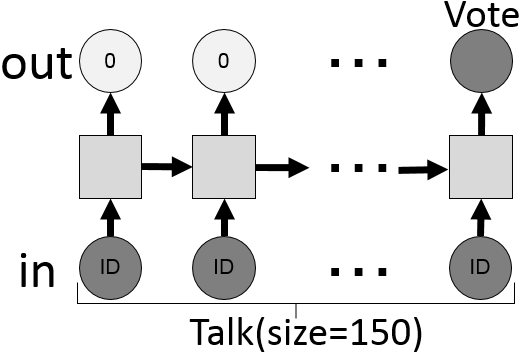
\includegraphics[width=6.0 cm]{./net.PNG}
  \end{center}
 \caption{学習ネットワーク \label{fig:net}}
 \end{figure}

\section{提案手法}
本稿では,ゲームログから得られる全プレイヤの会話情報を入力値とすることで,特定のプレイヤの投票先を予測することを試みる.\par
\subsection{ログデータ}
人狼知能プラットフォームver 0.3.5では,ゲームを実行すると終了時にゲームログを自動生成する仕様となっている.ゲームログには全フェーズの情報に加え,プレイヤの生死情報やエージェント名なども記載されている.\par
このゲームログから,学習の入力データとしてTalkフェーズの情報,出力データとしてVoteフェーズの情報を用いる.Talkフェーズのログには,一つの発言につき日付,ログ番号,発言者,内容,対象,役職 / 種族などの情報が,Voteフェーズには日付,投票者,投票対象の情報が記載されている.その中から,学習に使用するデータとして入力には発言者,内容,対象,役職 / 種族の4種類を用いる.また出力には,特定のプレイヤの投票先を予測するために投票者は固定して投票先のみを用いる.

\subsection{学習手法}
入力値には先述の情報をそのまま用いるのではなく,4種類を組み合わせたパターンそれぞれに与えたIDを用いる.教師値には投票先(1~15のプレイヤナンバ)を用いる.\par
ゲームでは各プレイヤは1日10回まで発言できる.したがって,プレイヤ人数は15人のため1日の全発言数は最大150となる.
図\ref{fig:net}に実験で用いるネットワークを示す.発言はひとつずつ入力していき,1~149個めの入力の際は教師値0として,150個めの発言を入力したときに教師値を投票先とする.モデルの更新は,1日の終了時にのみ行う.また,ゲーム進行に伴い死亡者が生じると,1日の全発言数は徐々に減っていくため,その際は入力値,教師値に-1を与えることで入力数を150に固定する.\par
以上のように1日の会話情報を入力,投票情報を出力として学習し,これをゲームが終わるかプレイヤが死亡する$n$日目まで繰り返す.なお,死亡者は予測時の選択肢から外すものとする.

\section{数値実験}
\subsection{実験内容}
実験に用いるデータとして,訓練用6500ゲーム,評価用6500ゲームを用意し,訓練時は100ゲーム65セットとして1エポックあたり1セットをランダムに学習した.表\ref{tb:param}に本実験のパラメータを示す.\par

\begin{table}[t]
    \begin{center}
    \caption{実験パラメータ    \label{tb:param}}
 \begin{tabular}{|c|c|}
 \hline
  エポック数&130\\
  \hline
  層&3層\\
  \hline
  中間ノード数&450\\
  \hline
  最適化手法&Adam\\
  \hline
  誤差関数&Soft\_max\_entropy\\
  \hline
 \end{tabular}
 \end{center}
\end{table}

また実験によって得られた投票先予測の正答率を評価する指標として,「Talkフェーズにおいて投票先の宣言をし,実際にそのとおりに投票する」という割合をHonestと定義し,それを用いた.ただし,JuN1roは狂人のアルゴリズムにおいて投票先を宣言しない,つまりHonestが常に0となるため,狂人のみ全評価時の1 /(評価時の生存人数 -1)の平均値をHonestとして用いることにする.(評価時の生存人数 -1)とは,投票候補者から自分を選択肢から外す動作である.\par

\subsection{実験結果}
学習の過程を記録したものとして,図\ref{fig:acc}に正答率Accuracy,図\ref{fig:loss}に誤差Lossのエポックごとの推移を示す.30~40エポック頃に変動が見られ,以後振動しながらも収束しているため,学習ができていることがわかる.\par
続いて表\ref{tb:ex}に学習が完了したモデルを評価用の6500ゲームに適用させた結果を示す.Accuracyは予測が的中した割合,Honestは先述の通り宣言した投票先に投票する割合を表す.

\subsection{検定}
実験結果について,Honestより高い精度で予測ができているかを確認するために二項検定をした.\par
検定統計量$T$は以下の式で表される.本検定において,標本比率$p$はAccuracy(正答数 / 評価回数),母平均$P_0$はHonest,標本数$n$は評価回数を示す.
\begin{eqnarray}
T = \frac{(p-P_0)}{\sqrt{\frac{(P_0(1-P_0))}{n}}}\nonumber
\end{eqnarray}
\hspace{1zw}帰無仮説を「AccuracyはHonestと差がない」とおき,有意水準$\alpha = 0.01$で各役職と全体の結果に対して両側検定したところ,村人,狂人および全体で帰無仮説が棄却された.したがって村人,狂人および全体において予測がHonestを上回ったことが言えた.


\begin{figure}[t]
  \begin{center}
  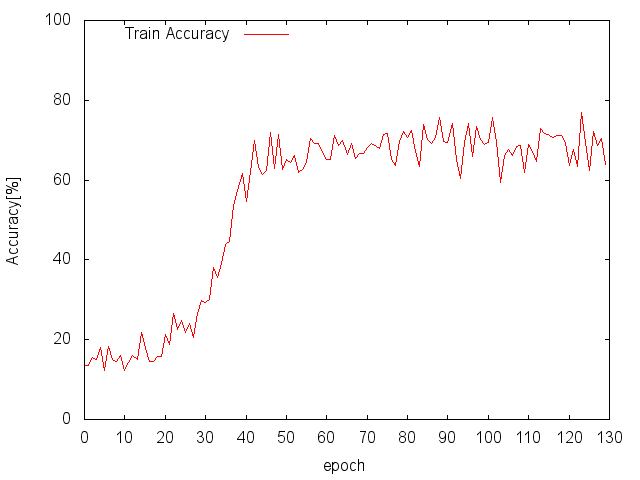
\includegraphics[width=7 cm]{./Accuracy.PNG}
  \end{center}
 \caption{Train Accuracy \label{fig:acc}}
 \end{figure}

\setlength\textfloatsep{15pt}
\begin{figure}[t]
  \begin{center}
  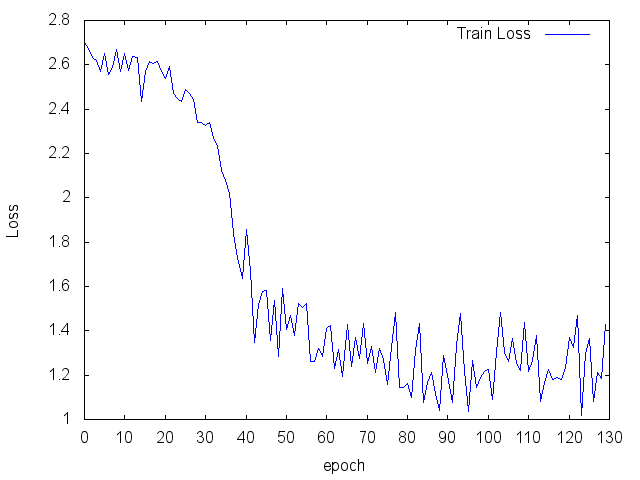
\includegraphics[width=7cm]{./Loss.PNG}
  \end{center}
 \caption{Train Loss \label{fig:loss}}
 \end{figure}


\setlength\textfloatsep{5pt}
\begin{table}[t]
    \begin{center}
    \caption{実験結果 \label{tb:ex}}
 \begin{tabular}{|c|c|c|c|}
 \hline
  役職&評価回数&Honest[\%]&Accuracy[\%]\\
  \hline \hline
  村人&14498&63.3&80.9\\
  \hline
  占い師&1300&98.5&97.6\\
  \hline
  霊媒師&925&70.0&72.2\\
  \hline
  狩人&2076&66.3&64.3\\
  \hline
  人狼&6721&45.5&45.6\\
  \hline
  狂人&1567&10.5&24.2\\
  \hline
  全体&27087&58.0&68.1\\
  \hline
 \end{tabular}
 \end{center}
\end{table}

\section{考察}
数値実験より,村人と狂人の場合はHonest以上の予測精度が得られたため,投票宣言以外の情報から投票先を予測できたと言える.予測において良い精度が出せたことの理由として,村人は誰を疑っているかを宣言するなど自らの思考を開示するアルゴリズムのため予測しやすかったと考えられる.また狂人は序盤に占い師を名乗ったプレイヤに投票することが多く,その傾向を捉えられたと推測できる.一方その他の役職では,村人のように思考を開示することがなく,狂人のような特殊な傾向も持たないため,予測しにくかったと考えられる.しかし概ねHonestと同程度の精度は得られており,投票宣言の傾向は捉えることができた.\par
役職ごとに見るとゲームで適用しうる成果が得られたのは村人のみであったが,村人はゲーム構成人数の過半数を占めるため,全体を考慮すると有用な結果が得られたと言える.\par

\section{まとめと今後の課題}
本稿では人狼エージェントが取る行動の一つである投票に焦点を当て,LSTMを利用して投票先を予測する手法を提案した.その結果,投票発言の傾向を捉えることができた.また,一部役職について投票発言のみによらない予測が実現し,全体として考慮したときにも有用な結果が得られた.\par
今後の課題として,精度の向上のために入力方法の再検討やLSTM以外の学習手法の適用を試みることが挙げられる.また本実験で用いたのはJuN1roのみのため,他のエージェントを利用した際の精度の検証も必要である.次の段階としては,投票先予測に加え役職や他の行動の予測をし,ゲーム全体の流れを把握することを目標とする.

%本稿では,人狼エージェントが取る行動の一つである投票に焦点を当て,LSTMを利用して投票先を予測する手法を提案した.その結果,投票発言の傾向を捉えることができた.また,一部役職について投票発言のみによらない予測が実現し,全体として見たときにも有用な結果が得られた.\par
%しかし思考を開示する発言や特殊な傾向がない場合,Honest以上の予測が難しいことが分かった.予測精度を向上させるためには,全プレイヤの投票情報や処刑対象者および襲撃対象者など,今回は用いなかった全プレイヤに開示されている情報などを加えて実験する必要がある.そのために,データの入力方法や学習手順も再検討しなければならない.\par
%今後の課題としては,本研究で用いたエージェントはJuN1roのみのため,他のエージェントセットを利用した際や複数のエージェントが混在したゲームにおける精度の検証が挙げられる.さらに,今回は時系列を考慮するためLSTMを利用したが,異なる学習手法を適用し,検討する必要がある.加えて,今回は投票先のみの予測であったが,襲撃先などActionの対象や役職の予測も試みて,今回の投票先予測と併用することで,ゲームの全体の流れを把握することを目指す.

\bibliographystyle{jabbrvunsrt}
\bibliography{index_ja}
\end{document}
% end of sci.tex
